\begin{figure*}[t]
\vskip 0.2in
\begin{center}


\includegraphics[width=0.8\columnwidth]{figures/pca_legend.pdf}

\subfigure{
{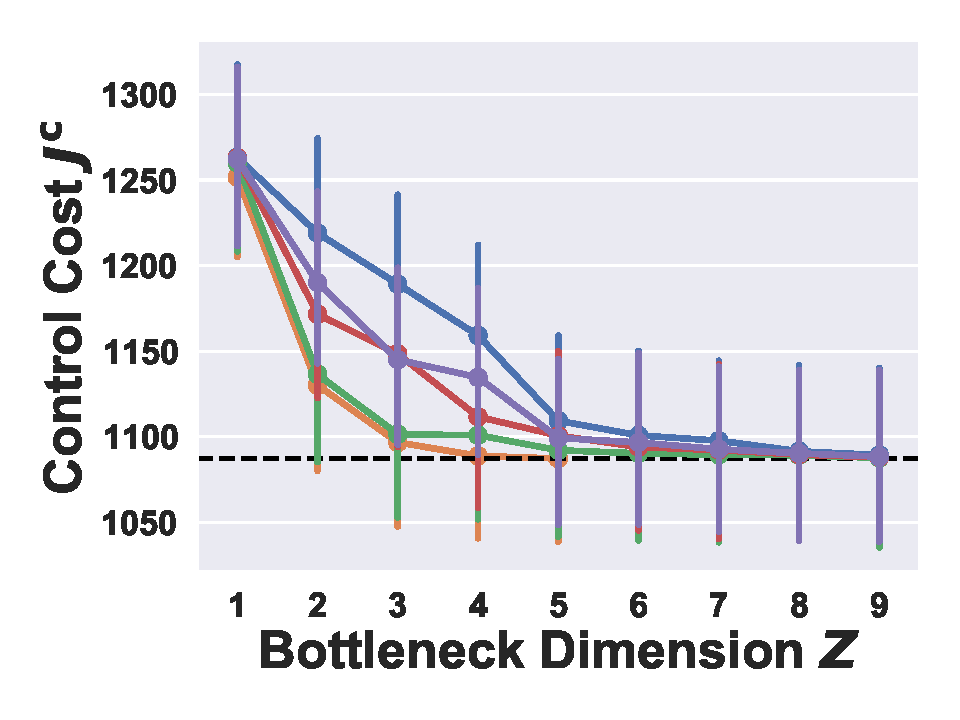
\includegraphics[width=0.4\columnwidth]{figures/pca/pca_mpc_cost_bottleneck.pdf}}
\label{fig_pca_cost_bottleneck}
}
\subfigure{
{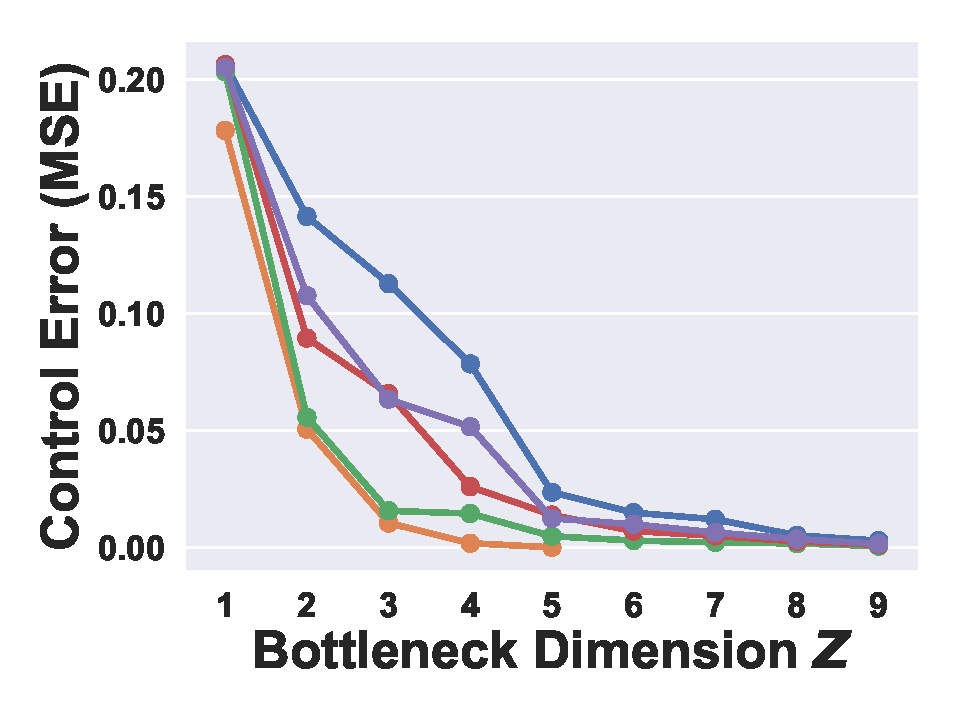
\includegraphics[width=0.4\columnwidth]{figures/pca/pca_mpc_ctrl_MSE.pdf}}
\label{fig_pca_ctrl_MSE}
}
\subfigure{
{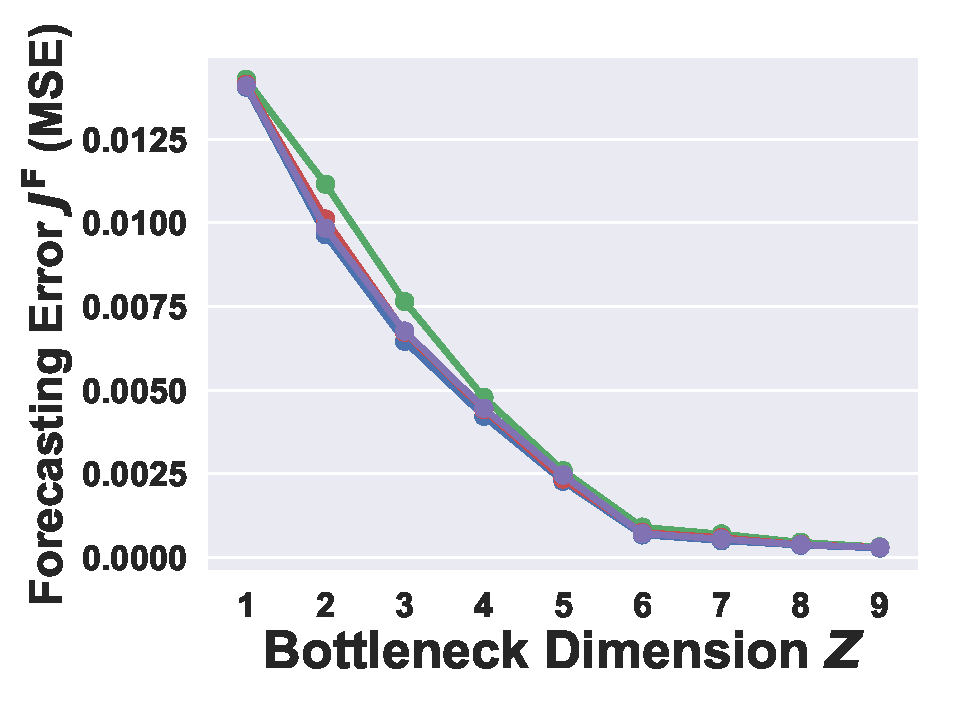
\includegraphics[width=0.4\columnwidth]{figures/pca/pca_mpc_fcst_MSE.pdf}}
\label{fig_pca_fcst_MSE}
}
\subfigure{
{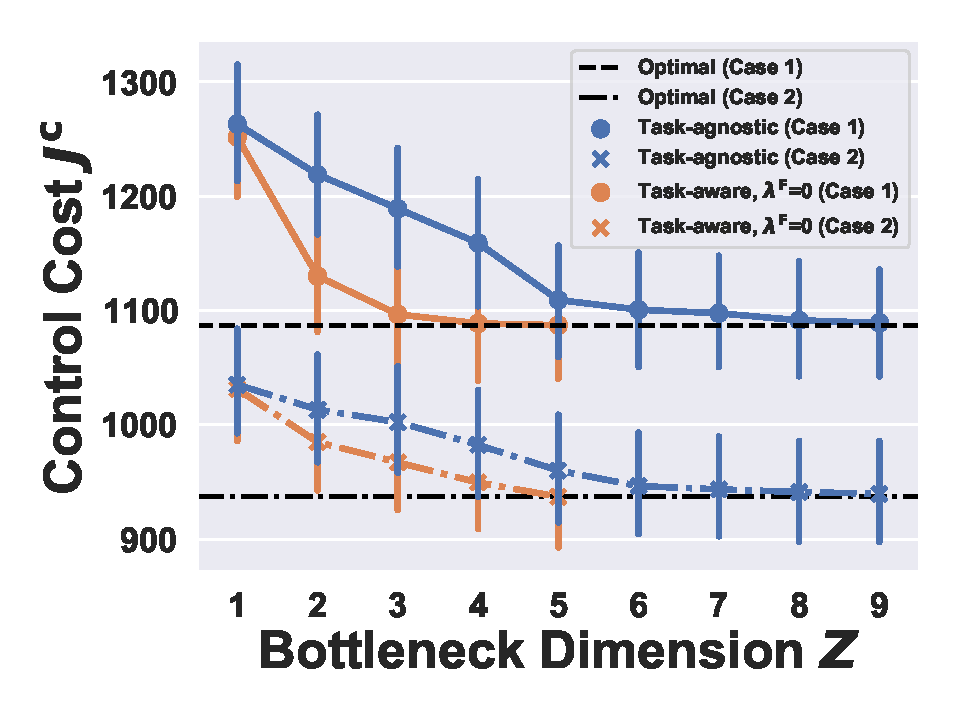
\includegraphics[width=0.4\columnwidth]{figures/pca/pca_cost_bottleneck_combined.pdf}
\label{fig_pca_forecast_errors}
}
}
\caption{\textbf{Linear control with MPC:} We repeat our analysis of input-driven LQR, but solve the problem in a receding horizon manner with forecasts for $H < T$ as discussed in Section \ref{subsec:input_driven_LQR} and Figure \ref{fig:main_pca_full}.
    (a) By only representing information salient to a control task, our co-design method (orange) achieves the optimal control cost with 
$60\%$ less data than a standard MSE approach (``task-agnostic'', blue). Formal definitions of all benchmarks are in Sec. \ref{sec:evaluation}. (b-c) By weighting prediction error by $\lambdaforecast > 0$, we learn representations that are compressible, have good predictive power, and lead to near-optimal control cost (\eg~ $\lambdaforecast=1.0$). The forecasting error of the task-aware scheme (orange) is much larger than the rest and thus not shown in the zoomed-in view.
(d) For the \textit{same} timeseries $\bolds$, two different control tasks require various amounts of data shared, motivating our task-centric representations.}
\label{fig:main_pca}
\end{center}
\vskip -0.2in
\end{figure*}
